\documentclass{article}
\usepackage[utf8]{inputenc}

\title{Graph Kernels and Support Vector Machines for Pattern Recognition}
\author{\textbf{Léo Andéol}\thanks{leo.andeol@gmail.com}\\ Master DAC, Sorbonne Université\\ Paris, France\\\\ \footnotesize Supervised by: Prof. Hichem Sahbi}
\date{May 2019}

\usepackage[square,sort,comma,numbers]{natbib}
\usepackage{graphicx}
\usepackage{amsmath,amsthm,amssymb}
\usepackage{mathtools}
\usepackage{multicol}
\usepackage{url}
\usepackage{todonotes}
\usepackage{lipsum}
\usepackage{apxproof}

\DeclarePairedDelimiter{\abs}{\lvert}{\rvert}
\DeclarePairedDelimiter{\norm}{\lVert}{\rVert}

\let\vec\mathbf
\newcommand*{\C}{%
  \mathbb{C}%
}
\newcommand*{\R}{%
  \mathbb{R}%
}
\newcommand*{\Z}{%
  \mathbb{Z}%
}

\newcommand*{\captionsource}[2]{%
	\caption[{#1}]{%
		#1%
		\\\hspace{\linewidth}%
		\textbf{Source:} #2%
	}%
}

\newtheorem{theorem}{Theorem}
\newtheoremrep{theorem}{Theorem}
\theoremstyle{definition}
\newtheorem{definition}{Definition}
\renewcommand{\putbib}{\listoffigures\listoftables\bibliographystyle{ieeetr}\bibliography{references}}
\renewcommand{\appendixbibliographystyle}{ieetr}
\renewcommand{\appendixbibliographyprelim}{\newpage}
\renewcommand{\appendixrefname}{References}

\begin{document}

\maketitle
\begin{abstract}
	The problem of having a framework to classify graphs is becoming increasingly important in the era of data. The issue has been tackled since the beginning of the millennium and there have been significant progress. This report introduces all necessary knowledge to understand the topic and then reviews different graph kernels while focusing on a random walk kernel and its optimization. Some experiments are then conducted to verify the information given by the state of the art, and some attempts are made to accelerate the different methods to compute the kernel.  
\end{abstract}

\newpage

\tableofcontents

\newpage

\section{Introduction}
 \paragraph{}Nowadays the world is shifting towards a new era where data is the most valuable resource, and researchers are working on algorithms to exploit it the best possible way. Most research is currently focused on the so-called "big data", huge quantities of data which are very sparse and of poor quality. However, there also exist structured databases of good quality, in the form of graphs, this different form being the one studied throughout this project. Graphs can be very useful in various fields, but are partly known for their use in biology, as they can be used to represent proteins or other types of molecules.
 \paragraph{}Classification of such graphs is an important problem of pattern recognition which affects a lot of sectors such as medicine, biology, and more. It was studied since the beginning of the millennium and significant progress has been made : several methods were discovered and gave good results but met a big issue, the complexity of these methods. Indeed, they do not scale well to large graphs as their complexity tends to be several times polynomial. Since then, the main objective of research on this topic has been to either find more computationally efficient algorithms, or to find methods to accelerate the ones already in use.
 \paragraph{}The first part of this report will introduce all the necessary background knowledge which are graphs as already mentioned, but also Support Vector Machines (SVMs) which is a powerful classification algorithm, and kernels which are transformations of data usually used to increase the accuracy of SVMs. However, graphs being non-vectorial data, kernels have also the purpose of becoming a metric of comparison between two instances of graphs. Thus, the main principles of graph kernels will be introduced as well as their definitions. Afterwards, the different methods used to improve the computation complexity of the kernel will be introduced together with their complexities, advantages and disadvantages.
\paragraph{}The second part of this report will be focused on the technical side and experiments conducted during the project. A synthetic graph database made of toy data was required to conduct simple and quick experiments. Indeed, it was made in order to verify the claims made in the main publication studied thanks to easy control on matters such as labeled and unlabeled graphs, and variations of the size of either the database or the graphs inside of it. Different challenges and problems met during the implementation will be explained, as well as their found solutions. Then, the main subject of this part will be discussed : the accuracy and computational time of different methods, estimation of their complexities and different attempts to approximate those methods. Finally, an experiment on a real dataset of mutagen molecules is conducted, and the results analyzed.

\newpage
\section{Methodology}
\subsection{Background}
\subsubsection{Graphs}
\paragraph{Definition}
A graph\cite{bondy1976graph} is a type of mathematical structure that represents connections between objects. It is more precisely an ordered pair $G=(V,E)$ of two sets: vertices $V$ (or nodes) and edges $E$ that connect two vertices together.
\begin{equation}
	E \subseteq \{(u,v) : (u,v) \in V^2\}
\end{equation}
Vertices represent objects and are usually depicted as circles or spheres whereas edges link pairs or vertices. 
\begin{figure}[!htb]
\begin{multicols}{2}
    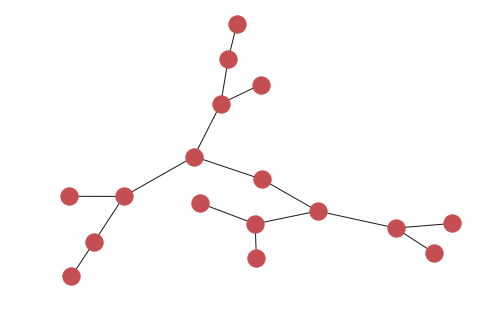
\includegraphics[width=\linewidth]{data/graphs/big_graph_no_label.png}\par
    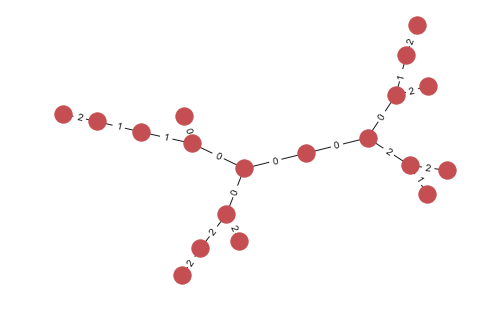
\includegraphics[width=\linewidth]{data/graphs/big_graph_label.png}\par
\end{multicols}
\caption{Two "tree" graphs, resp. unlabeled and labeled}
\end{figure}
\paragraph{Properties} Graphs have several different properties that will be used in the rest of this project and will be introduced here
\begin{itemize}
	\item A graph is undirected if and only if : $\forall (u,v) \in E \implies (v,u)\in E$
	\item $\abs{V}$ is the number of vertices and $\abs{E}$ the number of edges
	\item The degree of a vertex $d(v)$ is the number of vertices it is connected to, or the number of distinct edges connected to it.
	\item A path is a sequence of connected edges linking distinct vertices.
	\item A cycle is a path where the first and last vertex is the same.
	\item A graph can have labels (sometimes called colors) either on its vertices or edges (or both). They can take various forms such as integers, more generally elements of a finite or infinite set and even continuous (such as $\in \R$). 
	\item A graph is said to be connected if any vertex is connected, by a path, with any other vertex.
	\item An \emph{undirected} graph is a tree if there is exactly one path between any two vertices.
	\item A line graph $G'=(V',E')$ of a graph $G=(V,E)$ has a vertex for each edge $e\in E$ in $G$ and an edge $(u,v)\in V'^2$ if and only if there is a vertex in $G$ in common between the two former edges $u$ and $v$.
	\item A subgraph $G'=(V',E')$ of a graph $G=(V,E)$ is that graph restricted to a subset of nodes $V' \in V$ while keeping all the edges with those vertices $E' = \{(u,v) : (u,v) \in E \land (u,v) \in V'^{2}\} \subseteq E$
\end{itemize} The different methods studied in this report are focused on undirected graphs, either unlabeled or labeled by finite sets. Moreover, only edge-labeled graphs will be studied, thus if a graph is node-labeled, it can be transformed into an edge-labeled graph by computing its line graph.
\paragraph{Adjacency Matrix} The adjacency matrix of an undirected graph represents the presence or absence of an edge between two specific vertices. It is defined as the matrix $A$ of dimension $\abs{V}\times\abs{V}$ where entries are given by
\begin{equation}
	A_{i,j}=\left\{
	\begin{matrix}
	1 & \mbox{if } i \neq j \mbox{ and } (i,j) \in E \\
	0 & \mbox{otherwise}
	\end{matrix}
	\right.
\end{equation}

\paragraph{History} Graphs were first used in their modern form to represent the problem of Seven Bridges of Königsberg, and have been ever since used to represent maps, and thus path-finding algorithms were developed. They have also been used to represent flow problems, scheduling problems, networking routing and many others\cite{bondy1976graph}. Graphs can also be used, with labels, to represent different types of molecules and interactions between them, or more simply to represent molecules by considering atoms as vertices and bonds as edges.\\
The next part will introduce Support Vector Machines, the algorithm used in this project to classify new unknown graphs into known categories. It has been shown\cite{borgwardt_protein_2005} that it can be used effectively on proteins and enzymes.

\subsubsection{Support Vector Machines}
Support Vector Machines (SVMs)\cite{burges_tutorial_1998} are a type of machine learning algorithms discovered in the early 90s\cite{cortes_support-vector_1995}. It was originally a classification algorithm however it has been expanded since to regression and clustering too. 
\paragraph{Classification}
Classification is one of the two problems of supervised learning that aims to automatically recognize and classify observations, such as recognizing handwritten digits. It can be split into two tasks where the first one is to learn how to separate training data into classes using their attributes and the second is to predict the class of new examples. All of that, while minimizing errors. This problem can be formalized as
\begin{definition}
	Classification is the problem of associating observation data to a class. The training data comes as a set of observations and classes $\{(\vec{x_i},y_i)\}$ of size $N$ where $y_i \in \{-1,+1\}$, and using that data, an algorithm has to predict the class of new test data as accurately as possible.\\
	In other words, the objective is to find the best function $f :  \R^d \longrightarrow \{-1,+1\}$ among a set of functions $F$ while minimizing a risk function $R$
	\begin{equation}
		f\star = \mbox{argmin}_f R_{n}(f)
	\end{equation}
	 where $d$ is the number of features of the data .
\end{definition}
SVMs are especially powerful at this task and widely used for different reasons as explained subsequently.
\paragraph{Margin and support vectors}
The Support Vector Machines are based on the model of the Perceptron\cite{freund1999large}, another classification algorithm that tried to find a hyperplane that discriminates the two sets. The main issue with the Perceptron is that it has no formal guarantee to find an optimal hyperplane, and usually would not find it. Moreover, if the data are not linearly separable, the algorithm would not converge.\\
In order to tackle these issues, the SVM offered three solutions. First, a margin is added in the loss $L$ function in order to not only properly classify the data samples, but also with the maximum certainty, i.e. as far as possible from the decision boundary.
\begin{equation}
    \text{This loss is defined as : } L(y_i ,\vec{x}_i,w) = \max(0,1-y_i( \vec{x}_i\cdot \vec{w} + w_{0}))
\end{equation}
Where $\vec{x}$ is the feature vector of an instance, $y$ its class and $\vec{w}$ and $w_{0}$ respectively the weight vector and bias calculated by training the algorithm.
Considering this formulation is not sufficient, as there is an infinity of possible solutions. It is proven that the margin $\gamma$ between points and the decision boundary is inversely proportional to the norm of the weight vector $\norm{\vec{w}}$.\\
\begin{equation}
\gamma_i = \frac{y_{i}(\vec{x}_{i} \cdot \vec{w} + w_{0})}{\norm{\vec{w}}}
\end{equation}
These two solutions give us the first version the SVM, the hard-margin SVM\\ 
\begin{equation}
    \min_{\vec{w}} \frac{1}{2}\norm{\vec{w}}^{2} \quad
\textup{s.t.}\quad y_{i}(\vec{x}_{i} \cdot \vec{w} + w_{0}) \geq 1 \quad \forall i \in \{1..n\}
\end{equation}
However, if the data are not linearly separable the algorithm would not admit a solution since the quadratic programming problem requires all points to be correctly classified. Then, a new term $\xi$ is introduced as an error tolerance, as well as a factor $C$ that determines the balance between error tolerance and minimization of the weight vector norm $\norm{\vec{w}}$ :\\
\begin{equation}
\begin{array}{ll@{}ll}
\min_{\vec{w}}  & \frac{1}{2}\norm{\vec{w}}^{2}+C\sum\limits_{i=1}^{N}\xi_{i} &\\
\text{s.t.}& \forall i \in \{1..n\} & y_{i}(\vec{x}_{i} \cdot \vec{w} + w_{0}) \geq 1-\xi_{i}
\end{array}
\end{equation}
Then, the next section will introduce the second advantage of SVMs.
\subsubsection{Kernels}
In its dual form, the SVM problem only requires a dot product between the observation vectors. 
\begin{equation}
	\begin{array}{ll@{}ll}
	\max_{\alpha} & \sum\limits_{i=1}^{N} \alpha_i - \frac{1}{2} \sum\limits_{j=1}^{N}\sum\limits_{i=1}^{N}\alpha_{i}\alpha_{j}y_{i}y_{j}\vec{x_{i}}^{\top}\vec{x_{j}}\\
	\text{s.t.} & \forall i\qquad 0 \leq \alpha_{i} \leq C\\
	& \qquad \;\; \sum\limits_{i=1}^{n} \alpha_{i}y_{i}=0
	\end{array}
\end{equation}
Then, a nonlinear transformation $\phi(x)$ can be used to replace the dot-product $\vec{x}_i \cdot \vec{x}_j$ by $\phi(\vec{x_{i}})\cdot\phi(\vec{x}_{j})$ , effectively augmenting the dimensions of vectors from the input space into a higher dimensional feature space and thus the expressiveness of the model by enhancing the separability of the data. However, for complex transformations, such as in infinite dimensions, the function $\phi$ is not explicitly defined. But it was found\cite{cortes_support-vector_1995} that the standard dot products can be replaced by other functions as long as it positive semi definite. 
\begin{definition}
	A kernel $K$ is positive semi definite if and only if\\
    \begin{equation}
    	\sum\limits_{i=1}^{N}\sum\limits_{i=1}^{N}\kappa(\vec{x_{i}},\vec{x_{j}})c_{i}c_{j} \geq 0 \qquad \forall c_1\dots c_N \in \R^*
    \end{equation}
\end{definition}
Thus, the dot product can be replaced by a function $K(x_1,x_2)$ which will indirectly map the data to higher dimensions like the polynomial kernel(\ref{eq:pol}), even infinite with the RBF kernel (\ref{eq:rbf}) and return the dot product of those transformations, while remaining computable in all cases. This replacement is usually called the Kernel Trick. For example, the polynomial kernel is defined as follows
\begin{equation}
	\label{eq:pol}
	\kappa(\vec{x_{i}},\vec{x_{j}})=(\vec{x_{i}}^{\top}\vec{x_{j}}+c)^d
\end{equation}
where $d$ is the degree of the polynomial and $c$ the constant bias. Another example, the RBF kernel is defined as follows
\begin{equation}
	\label{eq:rbf}
	\kappa(\vec{x_{i}},\vec{x_{j}})={e}^{-\frac{\norm{\vec{x_{i}}-\vec{x_{j}}}^{2}}{2\sigma^{2}}}
\end{equation}
where $\sigma$ is a hyperparameter.
Ever since the foundation of SVMs, the kernel trick became a big focus of the machine learning community as it naturally fits in the algorithm and allows supervised learning on very complex data, and enjoying greater accuracy than most algorithms.\\
The fact that the dot product can be replaced by a function without specifying the map $\phi$ is the reason why the Kernel Trick became a big focus of research. In particular, it will be possible to make a kernel for non-vectorial data such as graphs, as shown in the next section. 
\subsection{State of the Art}
This section will review the state of the art kernels for graphs. Particular attention will be given to the random walk kernel.
\subsubsection{Graph Kernels}
Graph Kernels are a type of R-convolution kernels\cite{haussler99convolution} applied to graphs, which are kernels that are based on decompositions of complex objects and comparisons of those decompositions.\\
Graph Kernels have been studied since Support Vector Machines started getting popular\cite{kashima_graphkers_2003}. Since then, a lot of progress has been made, and several types of kernels have been discovered, such as random walk and graphlet\cite{shervashidze_efficient_2009} kernels, the two main families of kernels (and the ones studied in this section), but not the only ones.
There are also graph kernels that use subtrees\cite{ramon2003expressivity}, shortest paths\cite{borgwardt2005shortest} and several others that are unfortunately usually  either too complex to compute or not positive semi-definite\cite{shervashidze2012scalable}. However it has been shown\cite{schlkopf_learning_2001} that in some cases non positive semi definite kernels can still be used efficiently either by using them as a dissimilarity measure, or by artificially making them positive semi definite.
\subsubsection{Graphlets}
A graphlet is a small graph (with few nodes $k \leq 5$). The idea of the graphlet kernel $\kappa$ is to generate a set $S$ of all possible graphlets of a certain size $k$ and calculate for each of them the frequency of occurrence in a certain graph $G=(V,E)$ to build a vector $\vec{f}_G$ of dimension $\abs{S}$. The kernel is then defined as follows
\begin{definition}
	Let $G_1$ and $G_2$ be two graphs, ${\vec{f}_{G_{1}}}$ and $\vec{f}_{G_2}$ the frequency vectors of respectively $G$ and $G_2$, then the kernel $\kappa$ is defined as
	\begin{equation}
		\kappa(G_1,G_{2})=\vec{f}_{G_1}^{\top}\vec{f}_{G_2}
	\end{equation}
\end{definition}
However the complexity of computing this vector $\vec{f}_G$ is $O(n^k)$\cite{shervashidze_efficient_2009} where $n=\abs{V}$ and is thus computationally extremely expensive. In order to address this issue, a sampling method is introduced. Indeed, if enough samples are drawn, the Law of Large numbers indicates that the sampled distribution will converge to the actual (theoretical) distribution. However a bound has been found on the complexity of such sampling\cite{weissman2003inequalities} allowing better precision.
\subsubsection{Random Walks}
Graph kernels based on Random Walks have been studied since kernels started to be used on SVMs\cite{kashima_graphkers_2003}, several of them were discovered and then unified\cite{vishwanathan_graph_2010}. Random walks are a type of rather intuitive algorithms : the idea is to randomly walk through a graph and then compare it to random walks in another graph. Actually, given two graphs, the random walks are computed at the same time.\\
Moreover, it has also been shown\cite{imrich2000product} that performing a walk on two separate graphs at the same time is the same as performing a walk on the product graph. The product graph is in simpler the graph obtained by adding a vertex for each unique unordered pair of vertex of each graph, and adding an edge between two vertices if and only if there is an edge between those vertices in both graphs. The $vec$ operator will also be used as it is very linked to the tensor product. It is the vector obtained by stacking all columns of $A$. \\
\begin{definition}
	Let $G_1=(V_{1},E_{1})$ and $G_2=(V_{2},E_{2})$ be two graphs,\\the product graph
	$G_\times = (V_{\times},E_{\times})$ is then defined as
	\begin{itemize}
		\item $V_{\times} = \{(v,w) : v \in V_{1}, w \in V_{2} \}$
		\item $E_{\times} = \{((v_1,w_1),(v_2,w_2)) : v_1,v_2 \in V_{1}^2, w_1,w_2 \in V_{2}^2 \}$
	\end{itemize}
\end{definition}
For example, on very simple graphs, the following result is obtained
\begin{figure}[!htb]
	\begin{multicols}{3}
		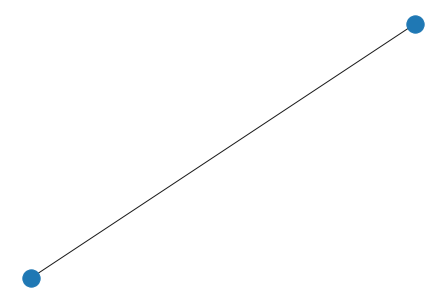
\includegraphics[width=\linewidth]{data/prod_graph/g1.png}
		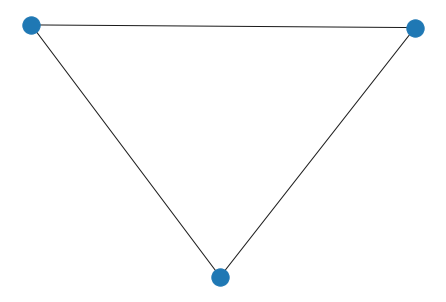
\includegraphics[width=\linewidth]{data/prod_graph/g2.png}
		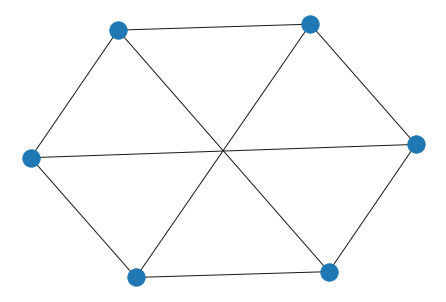
\includegraphics[width=\linewidth]{data/prod_graph/gx.png}
	\end{multicols}
	\caption{A graph $G_1$, a graph $G_2$ and the product graph $G_1 \otimes G_2$}
\end{figure}

However, technically, the adjacency matrix $W_{\times}$ of a such graph is the result of the Kronecker (tensor) product of the two adjacency matrices $A_1$ and $A_2$ of the two graphs \cite{weichsel1962kronecker}
\begin{equation}
    W_{\times}=A_1 \otimes A_{2}
\end{equation}
In case the graphs are labeled, then the adjacency matrix $W_{\times}$ is the sum of the Kronecker products of adjacency matrices restricted to each label $l$ 
\begin{equation}
	W_{\times}=\sum\limits_{l=1}^{d} A_1^{(l)} \otimes A_2^{(l)}
\end{equation}
Where $d$ is the size of the label set and $A^{(l)}$ the adjacency matrix of $G_x$ restricted to the label $l$ which is defined as follows
\begin{equation}
	A^{(l)}=\left\{
		\begin{matrix}
		1 & \mbox{if } i \neq j \mbox{ and } (i,j) \in E \mbox{ and } (i,j) \mbox{ is labeled } l\\
		0 & \mbox{otherwise}
		\end{matrix}
		\right.
\end{equation}

\paragraph{Kernel definition}
The idea of the kernel is to perform random walks simultaneously on two graphs in order to compare the walks they have in common. As shown above, this can be achieved by simply performing a random walk on the product graph.
By making the adjacency matrix stochastic, and computing the $k$-th power of the matrix $W_\times$, the probabilities obtained are the ones of walks in common (starting and ending at the same nodes) between the two graphs of length $k$.
By taking into account the start $p_\times$ and end $q_\times$ probabilities, the sum of walks of all possible lengths can be calculated. Moreover using a power series $\mu(k)$ helps de-emphasizing longer walks and makes the sum converge. 
\begin{definition}Let $p_{\times}$ and $q_{\times}$ be respectively the start and end probability of each node, and let $W_{\times}$ be the adjacency matrix of the product graph of $G$ and $G'$, and finally $\mu(k)$ be a convergent function of $k$, the random walk kernel is defined as\cite{vishwanathan_graph_2010}
	\begin{equation}
		\kappa(G_1,G_2) = \sum\limits_{k=0}^{\infty}\mu(k)q_{\times}^{\top}W_{\times}^{k}p_{\times}
	\end{equation}
\end{definition}
\noindent
This kernel can be computed in $O(kpn^6)$ with $k$ the the number of iterations and $p$ a constant which depends on the complexity of $\mu(k)$.
\paragraph{Inverse Kernel}
There is a specific case of the kernel provided that a power series is used. Indeed, by replacing the power series as follows $\mu(k)=\lambda^k$ the following kernel is obtained 
\begin{equation}
	\kappa(G_1,G_2)=q_{\times}^{\top}(I-\lambda W_\times)^{-1}p_{\times}
\end{equation}
It can also be computed in $O(n^6)$ however in practice the constant factor is much lower which makes it a better option for very small graphs and databases. Moreover, it will inspire some of the following acceleration methods.
\paragraph{Sylvester Equation}
A Sylvester equation, also sometimes called Lyapunov equation is a matrix equation of the following shape :
\begin{definition}
	Let $A$, $B$, and $C$ be matrices of compatible dimensions, then the discrete-time Sylvester Equation is 
	\begin{equation}
	AXB+C=X
	\end{equation}
	Which can be generalized as
	\begin{equation}
		\sum_{i=0}^{d}A_{i}XB_{i}+C=X
	\end{equation}
\end{definition}
These equations will be referred to as Sylvester Equation and Generalized Sylvester Equation. These equations are solved usually using Schur decompositions in $O(n^3)$ for the basic Sylvester equation and in unknown time for the generalized version\cite{vishwanathan_graph_2010}.\\
This equation can be used to compute the kernel faster assuming a geometric function $\mu(k)=\lambda^k$ with $\lambda$ an hyperparameter. It can be achieved by replacing the $A$ and $B$ matrices by the adjacency matrices $A_1$ and $A_2$, adding $\lambda$, and $C$ by the start probability vector $p_\times$ while vectorizing the whole equation thus obtaining
\begin{equation}
	vec(X) = vec(\lambda A_{1}XA_{2}) + p_{\times}
\end{equation}
From which the following can be obtained (where I is the identity matrix)
\begin{equation}
	q_{\times}^{\top}vec(X)=q_{\times}^{\top}(I-\lambda W_{\times})^{-1}p_{\times}
\end{equation}
Thus, having calculated the inverse kernel by an alternative method. The advantage of this method is that it is very fast and theoretically adapted to both labeled and unlabeled graphs. Moreover, compared to the others, this option is very simple and does not require specific parameters, but like many others, suffers when it encounters singular matrices.  
\paragraph{Conjugate Gradient Method}
The Conjugate Gradient Method\cite{nesterov_lectures_2018} is an optimization algorithm used to find approximate solutions of linear systems that have a positive semi definite matrix. As its name suggests, it is a gradient based iterative algorithm. The main idea is that normal gradient descent only takes into account the gradient at the current step of the algorithm, and depending on the step size may cancel progress made in the previous step.
\begin{figure}[!htb]
	\centering
	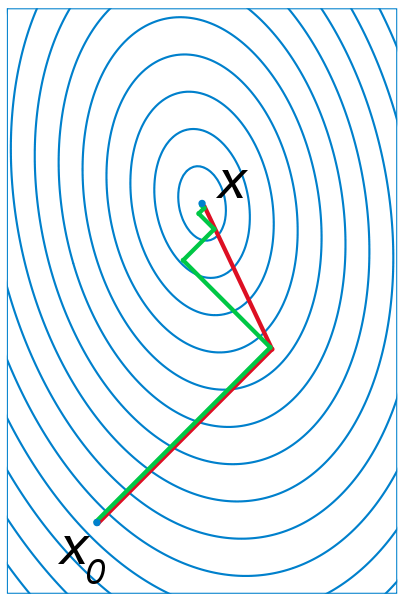
\includegraphics[height=0.3\textheight]{data/sota/conj_grad.png}
	\caption{Conjugate gradient (red) compared to Gradient Descent (green)}
	\label{fig:conj_grad}
\end{figure} 
The Conjugate Gradient method is introduced as a fix for that issue. The idea of the algorithm is to keep former gradients in order improve the convergence speed by making the new gradient orthogonal to all former ones through the Gram-Schmidt process, at each step. Thus, unless there are approximation errors, the algorithm guarantees convergence in $r$ steps, being the number of dimensions of the problem, here the size of the graph.\\
However, this algorithm has limitations, it can only be used to solve linear systems of equations as $Ax=b$ under the constraint that $A$ is symmetric positive definite.
In this case, the following algorithm can be used to solve the following problem 
\begin{equation}
	(I-\lambda W_{\times})x=p_{\times}
\end{equation}
And the kernel value can be obtained by computing $q_{\times}^{\top}x$. The complexity of that method is $O(rn^3)$ for unlabeled graphs and $O(rdn^3)$ for labeled graphs where $r$ is the effective rank of the matrix $W_{\times}$. It is important to note that this kernel also assumes a geometric $\mu(k)$ function. \\
This method is thus slower than the Sylvester Equation, however it is easily applied to labeled graphs, which is its main advantage.
\paragraph{Fixed Point Iterations}
A fixed point is a value for which a function, returns that same value 
\begin{definition}
	Let $S$ be a set and $f$ a map $f : S \rightarrow S$,\\
	$x \in S$ is a fixed point of $f$ if and only if $x=f(x)$ 
\end{definition}
Fixed point iterations is a method of computing a fixed point of a function by applying repeatedly the following equation until $\norm{x_{n+1}-x_{n}}<\epsilon$ where $\epsilon$ is the acceptable level of error.
\begin{equation}
	x_{n+1} = f(x_n)
\end{equation}
There is also a guarantee of convergence 
\begin{theoremrep}
	In order for the fixed-point iterations to converge, it is necessary that $\lambda<|\xi|^{-1}$ where $\xi$ is the largest eigenvalue of $W_\times$
\end{theoremrep}
\begin{proof}
  Let $x_0=p_\times$ and $t>>0$
  \begin{align*}
      x_{t+1}-x_t &= p_\times+\lambda W_{\times} x_t - x_t &\\
      &= p_{\times}+(\lambda W_{\times} - 1)(p_{\times}+\lambda W_{\times} x_{t-1})\\
      &= p_{\times} - p_{\times} + \lambda W_{\times}p_{\times} + (\lambda W_{\times})^2 x_{t-1} - \lambda W_{\times} x_{t-1}\\
      &= \lambda W_{\times}(p_{\times}-x_{t-1}+\lambda W_{\times} x_{t-1}) \\
      &= \lambda W_{\times}(p_{\times}-\lambda W_{\times} x_{t-2} - p_{\times} + \lambda W_{\times}(\lambda W_{\times} x_{t-2} +p_{\times}) \\
      &= \lambda W_{\times} ( \lambda W_{\times} (\lambda W_{\times} x_{t-2}+p_{\times}-x_{t-2})) \\
      &= (\lambda W_{\times})^2(\lambda W_{\times} x_{t-2}+p_{\times} - x_{t-2}) & \\
      \text{A pattern is found}\\
      \implies x_{t+1}-x_t &= (\lambda W_{\times})^t (\lambda W_{\times} x_0 + p_{\times} - x_0) & \\
      \text{And because } x_0 = p_{\times}\\
      &= (\lambda W_{\times})^{t+1} p_{\times}\\
      \text{Which decreases only when}\\
      \xi_1 < 1\\
      \text{The largest magnitude eigenvalue of} \lambda W_{\times}\\
      \implies \lambda < |\xi_1|^{-1}
      && \qedhere
  \end{align*}
\end{proof}
Since this method requires the computation of $W_\times$, the kernel value can be computed for any type of labeling. For unlabeled graphs, the complexity is $O(kn^3)$ and $O(kdn^3)$ for labeled graphs, where $d$ is the number of labels and $k$ the number of iterations which can be estimated by the following assuming that the contraction factor is $\lambda\xi_1$ with $\xi_1$ the largest eigenvalue of $W_\times$ :
\begin{equation}
	k=O\left(\frac{\ln \epsilon}{\ln \lambda + \ln \abs{\xi_1}}\right)
\end{equation}
Finally, the fixed point iterations is more demanding than the others since it has a condition on the value of $\lambda$ and thus assumes as geometric $\mu(k)$ function, and the number of iterations can easily vary a lot. The only advantage of this method is that it is very simple while still being better than the raw kernel.
\paragraph{Spectral Decomposition}
The Spectral Decomposition, usually called the eigendecomposition of a matrix $M$ is a factorization in the form $VDV^{-1}$ where $D$ is the diagonal matrix of eigenvalues and V the matrix of eigenvectors. This decomposition can reduce the computational time of the kernel by making most of the matrix operations trivial
\begin{equation}
	\kappa(G,G_2)=\sum\limits_{k=0}^{\infty}\mu(k)q_{\times}^{\top}(V_{\times}D_{\times}V_{\times}^{-1})^{k}p_{\times} = q_{\times}^{\top}V_{\times}\left(\sum\limits_{k=0}^{\infty}\mu(k)D_{\times}^{k}\right)V_{\times}^{-1}p_{\times}
\end{equation}
Indeed, the power now only applies to a diagonal matrix which can be computed much faster. Moreover, this method unlike the others preserves the prior $\mu(k)$ without any conditions. If $\mu(k)=\lambda^k$ is chosen then the kernel becomes
\begin{equation}
	\kappa(G,G_2)=q_{\times}^{\top}V_{\times}(I-\lambda D_{\times})^{-1}V_{\times}^{-1}p_{\times}
\end{equation}
That kernel is even more trivial to compute as the inverse of a diagonal matrix is simply the inverse of each of its entries and is thus computed in linear time. Finally, by using $\mu(k)=\frac{\lambda^k}{k!}$  as prior, the following new kernel is obtained
\begin{equation}
	\kappa(G,G_2)=q_{\times}^{\top}V_{\times}{e^{\lambda D_{\times}}}V_{\times}^{-1}p_{\times}
\end{equation}
However, the complexity of the computation of the eigendecomposition is as large as the raw kernel $O(pn^6)$, but, for unlabeled graphs, a big improvement is possible by simply calculating the eigendecompositions of the original adjacency matrices $A_1$ and $A_2$ thus cutting the time to $O(pn^3)$, thanks to a property of the Kronecker product
\begin{equation}
	A_1 \otimes A_2=(V_{1}D_{1}V_{1}^{-1})\otimes(V_{2}D_{2}V_{2}^{-1})=(V_1\otimes V_2)(D_1 \otimes D_2)(V_1 \otimes V_2)^{-1}
\end{equation}
By rewriting the spectral decomposition kernel taking advantage of this property, the following new kernel is obtained
\begin{equation}
	\kappa(G_1,G_2)=(q_{1}^{\top}V_{1}\otimes q_{2}^{\top}V_{2})(\sum\limits_{k=0}^{\infty}\mu(k)(D_{1}\otimes D_{2})^k)(V_{1}^{-1}p_{1}^{\top}\otimes V_{2}^{-1}p_{2}^{\top})
\end{equation}
Which can also be altered by choosing specific $\mu(k)$ as described above. This method ends up being the most efficient of all for unlabeled graphs as it is computed in $O(pn^2)$ where $p$ is the computational time of the power series $\mu$. Moreover this complexity can further improve the computational time of the gram matrix because the eigendecomposition of an adjacency matrix only needs to be computed once. However, this method cannot be expanded to labeled graphs as it encounters difficulties applying the property mentioned above.
\paragraph{Nearest Kronecker Product Approximation}
This method is more particular as it is not a new way to compute the kernel, but rather a way to generalize all the other methods. Indeed the Nearest Kronecker Product Approximation\cite{van1993approximation} is used to approximate two matrices $A$ and $B$ as if their Kronecker product if equal to the Kronecker product of two unlabeled graphs' adjacency matrices $W_{\times} \approx A \otimes B$. This methods allows using any of the methods mentioned above since it returns only two matrices and thus brings back the problem to unlabeled graphs. This method tries to minimize the Frobenius norm of the difference  $\norm{W_\times - A\otimes B}_F$. It can be computed in $O(dn^2)$ since $W_\times$ is a sum of Kronecker products, but since it is used in conjunction with other methods that are all in cubic time complexity, their overall complexity remains unchanged.\\
However this method also brings its own set of drawbacks. Since it required the Kronecker product of each couple of adjacency matrices to be computed, the previous advantage of the Spectral Decomposition (only computing once the eigendecomposition for each adjacency matrix) is lost as the obtained matrices are unique for each $W_\times$.

\subsubsection{Digest}
Several acceleration methods were introduced with various advantages and disadvantages. The following table sums up the most important attributes of each acceleration method.
\begin{table}[!htb]
	\begin{center}
		\begin{tabular}{|c|c|c||c|c||c|c|}
			\hline
			& \multicolumn{2}{c||}{Labels} & \multicolumn{2}{c||}{$\mu(k)$} & \multicolumn{2}{c|}{Complexity}\\
			\cline{2-7}
			Method & None & Finite Set & ${\lambda}^{k}$ & Any & Unlabeled & Labeled\\
			\hline
			Sylvester Equation & $\times$ & $\times$\footnotemark & $\times$ & & $O(n^3)$ & Unknown\\
			Conjugate Gradient & $\times$ & $\times$ & $\times$ & & $O(rn^3)$ & $O(rdn^3)$ \\
			Fixed Point Iterations& $\times$ & $\times$ & $\times$ & & $O(kn^3)$ & $O(kdn^3)$\\
			Spectral Decomposition& $\times$ & & $\times$ & $\times$ & $O(pn^3)$ & \\
			\hline
		\end{tabular}
	\end{center}
	\caption{Digest of the different properties of the aforementioned methods}
\end{table}\footnotetext{Theoretically\cite{lathauwer2004}}
The next section will be focused on experiments. It starts by introducing the framework used for this project and then analyzes the performances of those methods. 



\newpage
\section{Experiments}
A big part of this project consisted in implementing the different methods used to compute the random walk kernel\cite{vishwanathan_graph_2010}, verifying the results obtained in that article, and making new attempts to accelerate those algorithms while keeping the best accuracy possible.
\subsection{Databases and Metrics}
\subsubsection{A synthetic graph database}
In order to conduct experiments and verify claims made in the article, toy data is necessary. The first thing that had to be done is to create a graph database generator, of very simple and standard graphs that had predictable behaviors and could thus be used for standard tests. Those graphs would also be altered using simple transformations, in order to create different graphs belonging to the same class.
\begin{figure}[!htb]
	\begin{multicols}{4}
		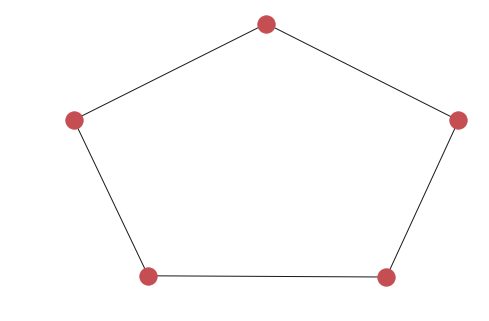
\includegraphics[width=\linewidth]{data/generated-graphs/ring_base.png}\par
		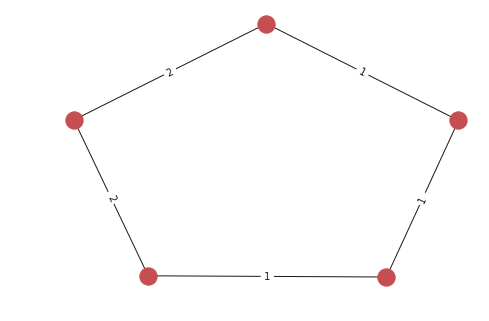
\includegraphics[width=\linewidth]{data/generated-graphs/ring_labels.png}\par
		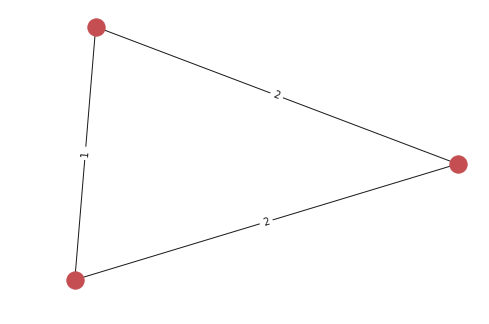
\includegraphics[width=\linewidth]{data/generated-graphs/ring_altered_struct.png}\par
		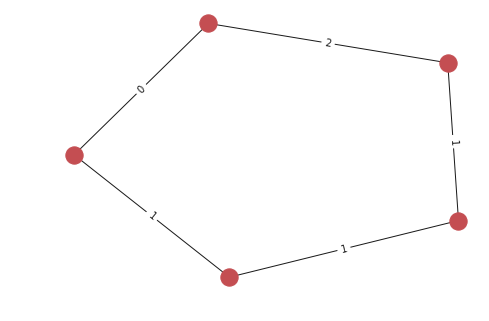
\includegraphics[width=\linewidth]{data/generated-graphs/ring_altered_labels.png}\par
	\end{multicols}
	\caption{Ring graphs, resp. unlabeled, labeled, altered structured, altered labels}
\end{figure}
For simplicity, it was decided to only use 3 classes. Focus is put on 3 standard types of graphs : the ring, the star and the tree. A ring graph is a connected graph where each vertex is connected to exactly two vertices, it thus forms one big cycle. A star graph is a particular tree-structured graph composed of a central node, and of several other nodes that are only connected to the central node, thus looking like stars in cartoon representations. Finally, a tree is a famous type of graph : it is a connected graph without any cycle, but here a special type of tree will be studied, since each vertex has a maximum degree of 3.
\begin{figure}[!htb]
	\begin{multicols}{4}
		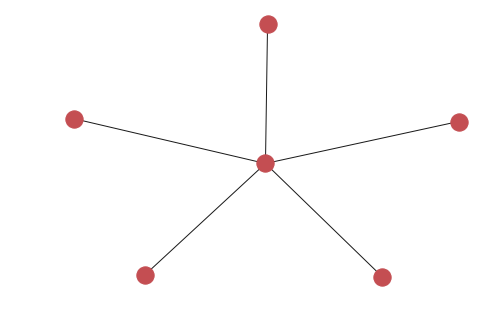
\includegraphics[width=\linewidth]{data/generated-graphs/star_base.png}\par
		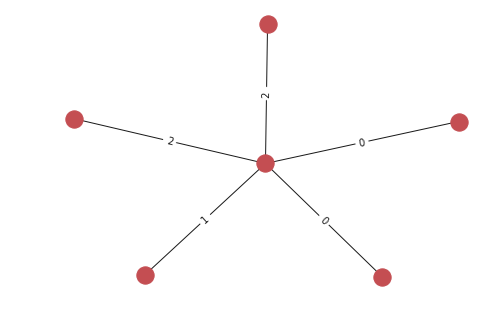
\includegraphics[width=\linewidth]{data/generated-graphs/star_labels.png}\par
		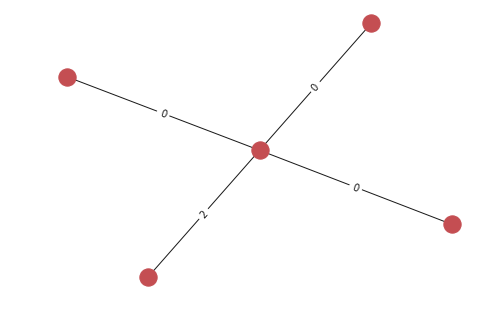
\includegraphics[width=\linewidth]{data/generated-graphs/star_altered_struct.png}\par
		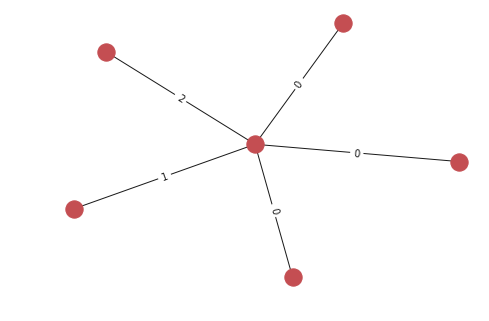
\includegraphics[width=\linewidth]{data/generated-graphs/star_altered_labels.png}\par
	\end{multicols}
	\caption{Star graphs, resp. unlabeled, labeled, altered structured, altered labels}
\end{figure}
Thus a synthetic graph database generator is created. For each type of graph, it creates a graph of predetermined size with randomly generated edge labels in a given interval. Then, for each graph, it alters it a predefined number of times, and each time creates a new graph that has been both altered on structure and on labels. Alteration on structure involves removing or adding a predefined number of nodes with respect to the type of the graph, the output graph being thus of the same class as the source. 
\begin{enumerate}
	\item Ring graphs are simply regenerated slightly longer or shorter, randomly.
	\item Star graphs are also regenerated either with more or less nodes, randomly.
	\item Tree graphs are either expanded by adding randomly leaves anywhere in the graph, or reduced by randomly removing leaves.
\end{enumerate}
Alteration on labels will randomly switch a predefined number of edge labels. Once this is done, the generator will create two databases out of the set of previously generated graphs, one will be made of the adjacency matrix of each graph without looking at labels, and the second one will be an array of adjacency matrices taken from graphs induced by selecting only edges with a specific label, and that for all labels in the label set.
\begin{figure}[!htb]
	\begin{multicols}{4}
		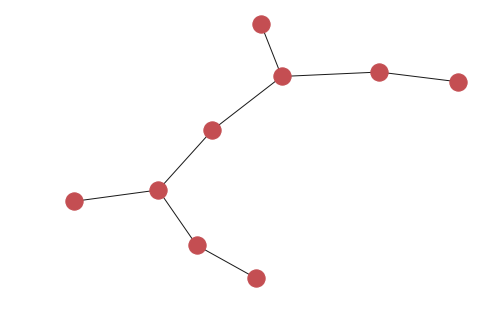
\includegraphics[width=\linewidth]{data/generated-graphs/tree_base.png}\par
		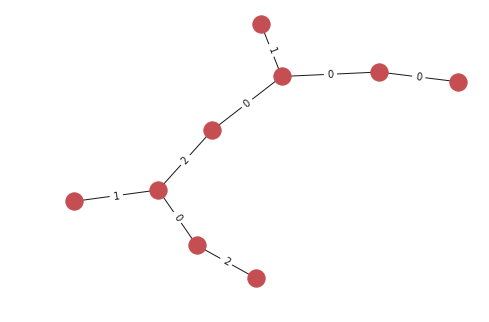
\includegraphics[width=\linewidth]{data/generated-graphs/tree_labels.png}\par
		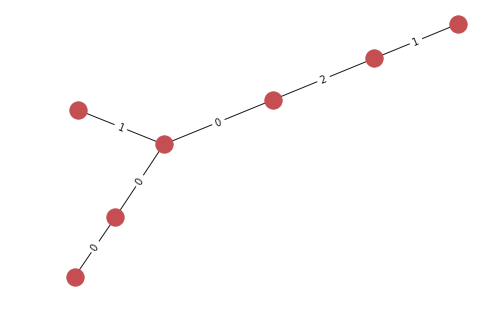
\includegraphics[width=\linewidth]{data/generated-graphs/tree_altered_struct.png}\par
		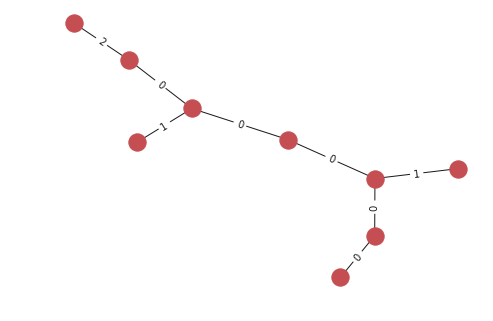
\includegraphics[width=\linewidth]{data/generated-graphs/tree_altered_labels.png}\par
	\end{multicols}
	\caption{Tree graphs, resp. unlabeled, labeled, altered structured, altered labels}
\end{figure}
\subsubsection{Real dataset}
After testing the different methods on synthetic data, they will be applied to a real dataset. The selected dataset is MUTAG, a dataset of chemical compounds. The objective for MUTAG is to classify the chemical compounds based on their mutagenic effect on bacterium.
\begin{table}[!htb]
	\begin{center}
		\begin{tabular}{|c|c|c|c|c|}
			\hline
			Dataset & size & classes & \# of vertices & \# of edges\\
			\hline
			%Enzymes & 600 & 6 & 33 & 124\\
			MUTAG & 188 & 2 & 18 & 39\\
			\hline
		\end{tabular}
	\end{center}
	\caption {Statistics on the real dataset}
	\label{tab:stats_real}
\end{table} Both accuracy and computational time will be analyzed in the Performance part, with focus being put the computational time.

\subsubsection{Metrics}
In the following experiments only two simple metrics will be used to compare the different methods. First, the accuracy is evaluated in a given set $X$ simply using the 0-1 loss function as follows
\begin{equation}
L(X,\vec{y})=\frac{1}{\abs{X}}\sum\limits_{i=1}^{\abs{X}}\left\{
\begin{matrix}
1 & \mbox{if } f(\vec{x}_i) \neq y_i \\
0 & \mbox{otherwise}
\end{matrix}
\right.
\end{equation}
This function gives the rate of prediction errors on test data in $X$ since the classes are balanced.\\
The second metric used is the computational time, expressed in seconds. 
\subsection{Evaluation Protocols}
Implementing code from the main paper is a challenge in itself. Several problems are not really documented and finding functions to solve them, or even explanations on how to solve them is sometimes difficult.
\paragraph{Support Vector Machines}
The Support Vector Machines algorithm is not implemented since it is not the focus of this project. Instead, the famous library libsvm\cite{cc2011libsvm} is used through the python library scikit-learn\cite{pedregosa2011scikit} because of its efficiency and renown. Moreover, there are some hyperparameters to optimize, namely the penalty coefficient on classification mistakes $C$. Several experiments on various databases show that the penalty coefficient $C$ had virtually no effect on the accuracy, thus was kept at a value of 1.
\paragraph{Gram Matrix}
The SVM library used in the project allows us to precompute the kernel and feeding it to the algorithm. This kernel matrix is called a gram matrix where its entries $M_{i,j}\in [0,1]$ represent the similarity between $G_i$ and $G_j$. Thus this matrix is obviously symmetric and it is only required to compute approximately half of the entries (precisely $\frac{n^2+n}{2}$).
\paragraph{Raw Kernel}
The Raw Kernel is very simple to implement however encounters an issue : a sum to infinity cannot be computed as-is, and thus a choice had to be made. It is decided that the raw kernel would be computed over $T$ iterations where $T$ would be the number of vertices of the largest graph. Moreover it was also decided to use the aforementioned power series $\mu(k)=\lambda^k$ to be able to compare results with the other methods restricted to it. The advantage is that all graph kernel values would be computed with the same number of iterations and the number of iterations would be kept small while all vertices would be reachable from any other vertex (the shortest path between two vertices in a connected graph $G=(V,E)$ is at most $\abs{V}$ long).  
\paragraph{Inverse Kernel}
This kernel is also very simple to implement  since it only required computing $I-\lambda W_{\times}$ and its inverse, which is handled exclusively by numpy (part of the scipy project).
\paragraph{Sylvester Equation}
The Sylvester Equation is a good example of poorly documented problems (compared to the others). There are very few resources on the subject, and even less implementation of solvers. The Sylvester Equation could theoretically be used on both unlabeled and discrete-labeled graphs which are respectively represented as Sylvester and Generalized Sylvester Equations (involving a sum of matrices), however, the only library available so far solves the first one, but not the second one. There seems to be confusing terminology since there is a solver for the Generalized Sylvester Equation, but a different one than the one described in the studied source\cite{vishwanathan_graph_2010}. The same source also mentions a way to solve the generalized version\cite{lathauwer2004}, however, this option is not explored because of a lack of time.  
\paragraph{Conjugate Gradient Method}
The Conjugate Gradient Method is however very well documented\cite{nesterov_lectures_2018} and there are several libraries implementing this algorithm. Since the main library in python\cite{jones2016scipy} only implemented this method on sparse matrices, it gave very poor computational time efficiency on the synthetic database. It was then decided to implement it directly and gave much better results. As said previously, the algorithm guarantees convergence in $r$ step where $r$ is the effective rank of the matrix $I-\lambda W_\times$. 
\begin{figure}[!htb]
	\centering
	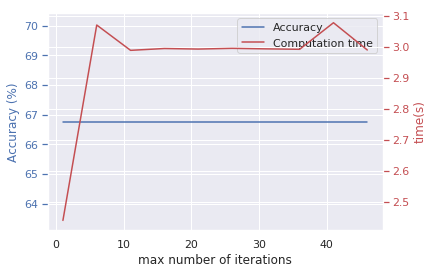
\includegraphics[width=0.7\linewidth]{data/conj_grad/acc_time_fct_iter.png}
	\caption{Accuracy and computational time depending on number of maximum iterations}
\end{figure}
However, by grid search on the maximum number of iterations allowed for the algorithm, it was discovered that on synthetic data the effective rank of the matrices is very low and the algorithm converges very quickly. This can be caused by the fact that the synthetic database is too simple and the adjacency matrices too sparse, making the problem too easy to solve.
\paragraph{Fixed Point Iterations}
The Fixed Point Iterations method is very easy to implement since the algorithm only consists in repeating $x_{t+1}=p_{\times}+\lambda W_{\times}x_t$ until either convergence is obtained or the maximum number of iterations reached. It rapidly gave good results thus being used as a tool of comparison with other kernels that struggled more at the beginning.
\begin{figure}[!htb]
	\centering
	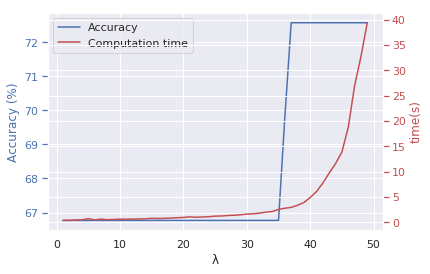
\includegraphics[width=0.7\linewidth]{data/fixed_point/acc_comp_time_fct_lambda.png}
	\caption{Accuracy and computational time depending on chosen $\lambda$}
\end{figure}
However there is a constraint on the lambda (the geometric factor) used in the kernel as proved above. Experiments showed that a lambda very close to the constraint increases significantly the time of computation to convergence, as well as the density of the adjacency matrix to a lower extent.

\paragraph{Spectral Decomposition}
The Spectral Decomposition method is also very well documented since it is simply another name for the eigendecomposition, one of the main problems of linear algebra. Because of that it is very simple to implement since the method only requires Kronecker products and inverses. However, the fact that several inversions are required can lead to an accumulation of numerical imprecisions. Moreover, in some other cases the left eigenvectors matrix is singular and is not invertible. In order to fix that, an $\epsilon$ was added to all the diagonal of the adjacency matrices such that it would not alter the results (and did not) while allowing all kernels to be computed. Finally, the chosen $\mu(k)$ function is the power series to keep the method comparable to others.
\paragraph{Nearest Kronecker Product}
The Nearest Kronecker Product Approximation (NKP)\cite{van1993approximation} is used in conjunction with others methods in order to make them compatible with labeled graphs, it is especially useful with the spectral decomposition which is theoretically the fastest method available. There is some documentation on the topic however it is relatively hard to get a good grasp on the topic. Thus, a simple version of the NKP is implemented that does not take into account the special property of the product graph being composed of a sum of Kronecker products, making the overall complexity $O(n^3)$ instead of $O(dn^2)$.
	

\subsection{Performance}
First of all the different methods will be tested with synthetic data to verify claims made in the report. Then, the methods will be applied to real world problems. 
\subsubsection{Performance on synthetic data}
\paragraph{Gram Matrices}
The algorithms approximate the kernel using very different techniques, thus the gram matrices obtained from the kernels were similar in appearance, but had significant differences of scale. It was then decided to normalize very simply the gram matrices so they could be more easily compared.
\begin{equation}
M = (M - min(M))/(max(M) - min(M))
\end{equation}
\begin{figure}[!htb]
	\begin{multicols}{3}
		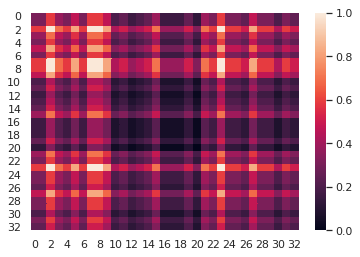
\includegraphics[width=\linewidth]{data/gram/gram3.png}\par
		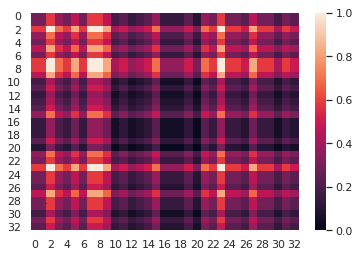
\includegraphics[width=\linewidth]{data/gram/gram4.png}\par
		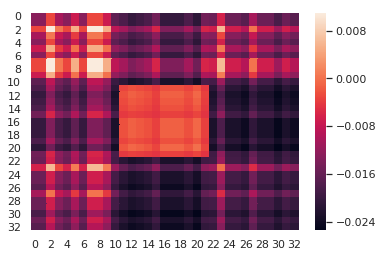
\includegraphics[width=\linewidth]{data/gram/gram5.png}\par
	\end{multicols}
	\caption{A gram matrix computed with the raw method, another with the fixed point method, and the difference between the second and the first}
\end{figure}
First, it should be noted that the scales vary largely, as the first two matrices have entries in $[0,1]$ and the difference in $[-0.024,0.008]$. It can be seen that the two matrices are indeed very similar, but locally there can be significant differences. The difference matrix shows that the fixed point kernel has higher values on the three diagonal blocks in average, and in average also, less in the outer parts of the matrix. Since in this example the data is ordered by class, it shows that the fixed point method gives in average higher values to graphs of the same class and smaller values to graphs of different classes than the raw method. It can be conjectured that the fixed point method will give a better accuracy, which is verified empirically in another paragraph.
Afterwards, in order to verify all the algorithms gave similar results, it was decided to compute the Frobenius norm of the difference of two gram matrices (divided by the size of the matrix, thus giving the mean squared error of any entry). The following results were obtained and were satisfying.
\begin{table}[!htb]
	\begin{center}
		\begin{tabular}{|c|p{12mm}|p{13mm}|p{15mm}|p{15mm}|p{15mm}|p{13mm}|}
			\hline
			& Raw\newline kernel & Inverse\newline Kernel & Sylvester\newline Equation & Conjugate\newline Gradients & Fixed\newline points & Spectral\newline Decomp. \\
			\hline
			Raw. & 0 & 1.1e-4 & 9.8e-5 & 8.9e-5 & 1.0e-4 & 1.0e-04  \\
			\hline
			Inv. & - & 0 & 2.1e-5 & 7.9e-5 & 4.0e-6 & 6.8e-6 \\
			\hline
			Syl. & - & - & 0 & 8.0e-5 & 1.7e-5 & 1.4e-5  \\
			\hline
			Con. & - & - & - & 0 & 7.9e-5 & 7.9e-5  \\
			\hline
			Fix. & - & - & - & - & 0 & 2.8e-6 \\
			\hline
			Spe. & - & - & - & - & - & 0 \\
			\hline
		\end{tabular}
	\end{center}
	\caption {Mean squared error of matrix entries}
	\label{tab:frobenius_norm_diff} 
\end{table}
Indeed, the mean squared error is small in most cases so that the different acceleration methods are probably going to give approximately correct results.
\paragraph{Label Use}
The synthetic database generates at the same time adjacency matrices of each graph, and the list of adjacency matrices filtered by each label. Thus, the scores obtained for each of the metrics can be compared, computed using the fixed point kernel since it is both fast and allows the use of labels.
\begin{figure}[!htb]
	\begin{multicols}{2}
		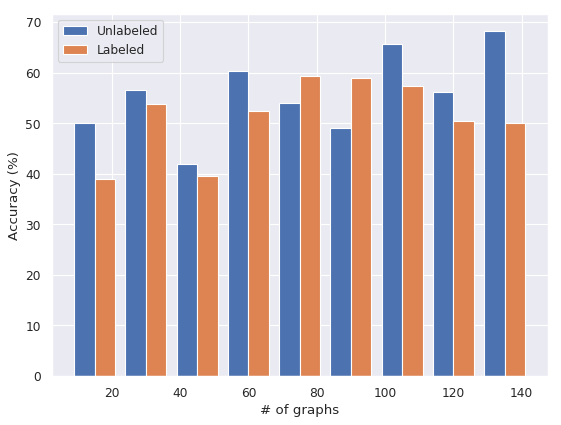
\includegraphics[width=\linewidth]{data/lab_nolab/acc.png}\par
		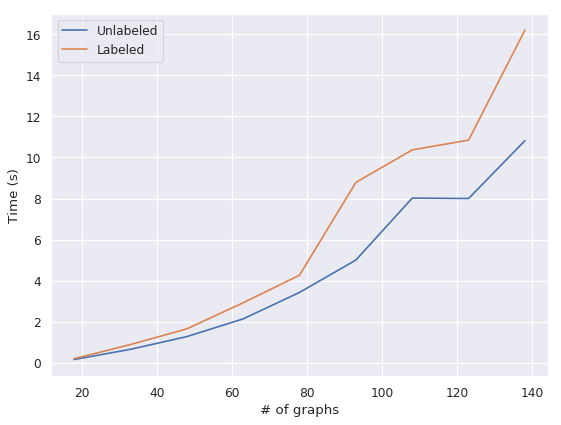
\includegraphics[width=\linewidth]{data/lab_nolab/time.png}\par
	\end{multicols}
\caption {Accuracy and computational time of learning for unlabeled and labeled graphs}
\end{figure}
Overall in most cases the unlabeled version gives better accuracy which can probably be explained by the fact that the graphs used in the experiments are not big enough with a set of labels too large, and thus a small change on labels could have a big effect on the kernel, for example on the central edge of a tree graph. It is conjectured that provided a large and connected enough graph, a small change in label does not alter much its list of adjacency matrices, labels will have a positive impact on the accuracy. Concerning the computational time, the difference is quite small though by increasing the size of the database the difference can be better observed. There is a small factor of difference during the computation of the tensor product.
\paragraph{Comparison of methods depending on the number of graphs}
This method is rather different from the others. Indeed, the variable in this experiment, the number of graphs, does not directly impact the complexity of the different methods. It is actually used to enhance the visibility on the differences of complexity between the methods at a given point. Thus, it confirms that the raw random walk and inverse kernel evolve jointly, as the 4 others evolve jointly too. 
\begin{figure}[!htb]
	\centering
	%\begin{multicols}{1}
		%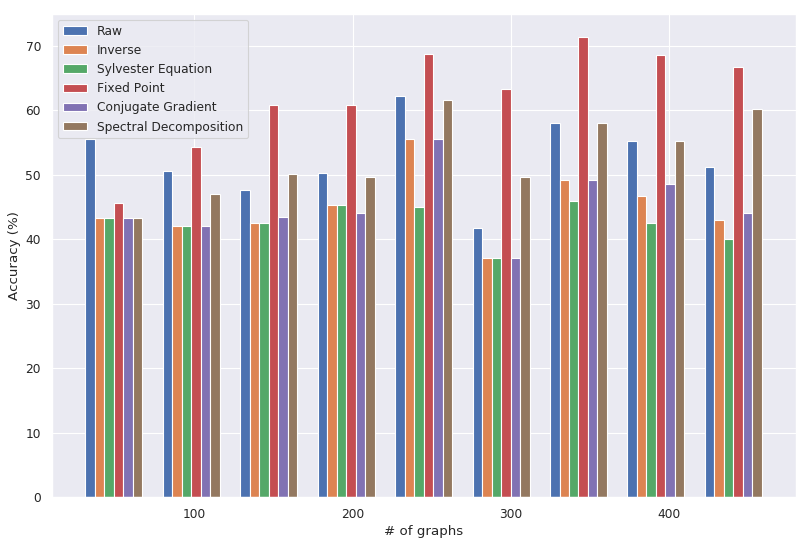
\includegraphics[width=\linewidth]{data/nb_graph/acc.png}\par
		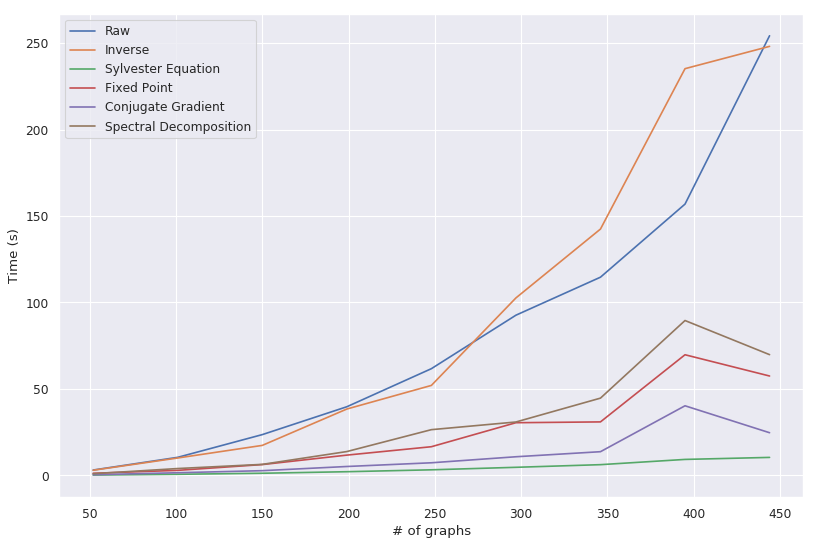
\includegraphics[width=.5\linewidth]{data/nb_graph/time.png}\par
	%\end{multicols}
	\caption{Computational time of different methods depending on the size of the database}
\end{figure}

\paragraph{Comparison of methods depending on the number of nodes}
In order to verify the complexities of the acceleration methods introduced above and compare their efficiency, their accuracy and computational time were calculated on synthetic databases with graphs of varying sizes. The databases were generated independently, thus the experiments of different sizes should not be compared in absolute values but rather relative. However, being generated following the same precise rules, the deviation is not too large.
\begin{figure}[!htb]
	\begin{multicols}{2}
		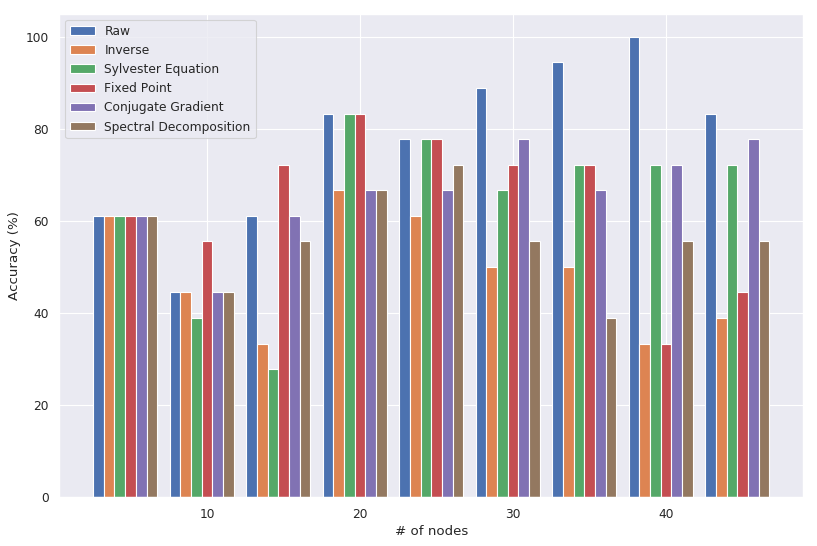
\includegraphics[width=\linewidth]{data/nb_nodes/acc.png}\par
		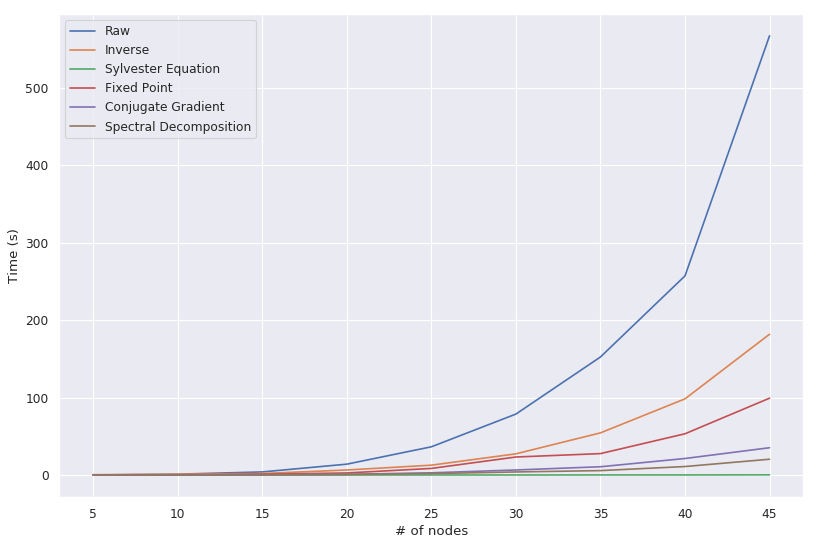
\includegraphics[width=\linewidth]{data/nb_nodes/time.png}\par
	\end{multicols}
\caption{Accuracy and Computational time of different methods depending on the size of graphs}
\end{figure}
Concerning the accuracy, the conjecture on fixed point accuracy made earlier is verified in most cases : the fixed point method gives the best approximation of the raw kernel, albeit at the cost of higher computational time. It can be also noted that the raw kernel method is rarely beaten, only once by the fixed point kernel only. Surprisingly the inverse method is in average the worst performing, all the other methods approximating it giving better results than it. Finally, the Spectral Decomposition method gives disappointing results, which can be explained by the accumulation of numerical imprecisions.\\
On the other hand, concerning computational time, it is important to remind that in this case some methods (fixed point, conjugate gradient) were implemented entirely for this project, while the Spectral Decomposition and Inverse methods used tools to compute eigenvalues and inverses, and finally the Sylvester Equation solver is taken from a library based in Fortran. This library is probably a lot more optimized than my personal code and thus may be the cause of a bias in computational time.\\
The difference of time complexity between the raw method, the inverse method and others is very noticeable and thus the acceleration methods are very time efficient. The most particular case is again the fixed point method which has a complexity increasing much faster than other methods, which could be explained by the number of iterations being much higher than the conjugate gradient for example, and thus computing the matrix vector products several more times, which is correlated to the error tolerance chosen for the fixed point iterations.
\paragraph{Nearest Kronecker Product}
This method is to be used in conjunction to other methods in order to adapt them to unlabeled graphs. It has been implemented as specified earlier, in a non-optimal manner ($O(n^3)$) but gave good results. 
\begin{figure}[!htb]
	\begin{multicols}{2}
		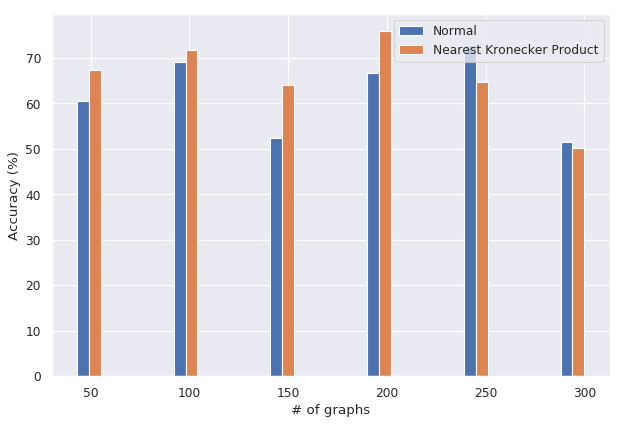
\includegraphics[width=\linewidth]{data/nkp/acc.png}\par
		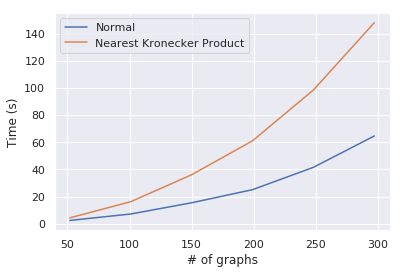
\includegraphics[width=\linewidth]{data/nkp/time.png}\par
	\end{multicols}
\caption{Accuracy and Computational time comparison between using a labeled database and the Nearest Kronecker Product Approximation}
\end{figure}Indeed, the accuracy obtained by approximating the Kronecker product from two labeled graphs has virtually the same values as the original one, taking variations into account. Moreover, the computational time is slightly increased, which can probably be explained by the fact as precised before, that the method implemented is the general NKP in $O(n^3)$ and not the specific case for sums of Kronecker products in $O(dn^2)$, thus effectively multiplying the complexity of the method used by a constant, since all methods are in $O(n^3)$.\\
In order to visualize the approximation better, two gram matrices were computed on the same dataset, the first one using the product adjacency matrix of labeled graphs, and the second one computed using the NKP and thus approximating the first. It can be seen that the matrices are very similar, the first one being more clear with less monotonic changes between its entries, and the second being a lot smoother in its transitions, induced by the noise caused by the selections done on singular values in the algorithm.
\begin{figure}[!htb]
	\begin{multicols}{2}
		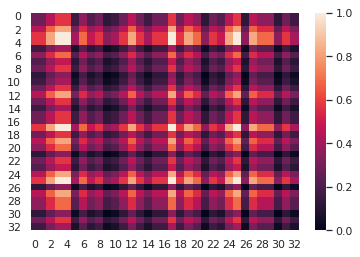
\includegraphics[width=\linewidth]{data/nkp/gram.png}\par
		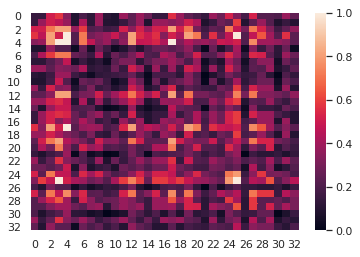
\includegraphics[width=\linewidth]{data/nkp/gram_approx.png}\par
	\end{multicols}
\caption{Two gram matrices computed resp. using labeled graphs and using the NKP of those graphs}
\end{figure}

\subsubsection{Performance on real datasets}
This implementation is also tested on a real database, which is MUTAG. First of all, the computational time bias on the Sylvester Method seems to appear also here, where its computational time relative to the others does not match with previous studies\cite{vishwanathan_graph_2010,shervashidze_efficient_2009}. Then, the different accuracies obtained  on MUTAG are even as good as the best results of a previous study using Graphlets \cite{shervashidze_efficient_2009}, and much better than their random walk kernel. The only exception is the Spectral Decomposition kernel which involves several operations subject to numerical imprecisions as said before.
\begin{table}[!htb]
	\begin{center}
		\begin{tabular}{|c||c|c|}
			\hline
			& \multicolumn{2}{|c|}{MUTAG}\\
			%%% nb of graphs
			\cline{2-3}
			Method & Accuracy & Comp. time\\
			\hline 
			Raw Kernel & $83.9\pm 3.1$ & 1'54"\\
			Sylvester Equation & $83.5\pm 2.8$ & 5"\\
			Conjugate Gradient & $83.5\pm 2.8$ & 18"\\
			Fixed Point Iterations & $83.5\pm 2.8$ & 47" \\
			Spectral Decomposition & $82.4\pm 1.3$ & 43"\\
			\hline
		\end{tabular}
	\end{center}
\caption{Classification accuracy in percent \% with standard deviation and computational time for each acceleration method on the MUTAG dataset}
\end{table}
Concerning the computational times, the Sylvester equation method and the Conjugate Gradient method are the two best performing, compared to the fixed point iterations which takes too many steps to converge in this case. Finally, the Spectral Decomposition method is less efficient than expected, which is linked to the fact that the eigendecompositions are computed twice for every pair of graphs, which is computationally expensive. 

\section{Conclusion and Future Work}
\paragraph{Conclusion}
In this project, different graph kernels were introduced, and focus was put on the random walk kernel, which is computationally expensive ($O(n^6)$). Thus, several acceleration methods were introduced in order to lower the complexity to a more acceptable bound $O(n^3)$, the lowest found yet. Another method, the Nearest Kronecker product was also introduced to enable any acceleration method to compute the kernel on labeled graphs by approximating them as unlabeled graphs. The computational time is lowered, but at the likely expense of a loss in accuracy.\\
In order to experiment with these methods, a synthetic database was created, and a real dataset used. After having solved some implementations issues, experiments were lead on these methods. It was shown that the computational time of the fixed point iterations wildly increases when $\lambda$ is in the neighborhood of the inverse of the matrix's largest eigenvalue. It also was shown that the number of iterations of the conjugate gradient had virtually no impact on the synthetic database beyond very small values.\\
Then, the complexity of the different methods was verified, by computing them on a synthetic database composed of graphs of different sizes. The accuracy of the Nearest Kronecker Product was tested on the synthetic database with similar levels of accuracy reached. Finally, the different methods were tested on the real dataset and gave good to better results than previous studies.
\paragraph{Future Work}
Some options in this project were not explored by lack of time, especially two, one theoretical, another slightly more technical. The first option is to generalize the Spectral Decomposition method to labeled graphs, as it is the fastest method theoretically and the only one that can be combined with any weighting function, it would become the best option in any scenario. The second option is to work on an algorithm to solve the Generalized Sylvester Equation so that it can also be applied to labeled graphs in practice, but also finding its complexity, which is unknown as of latest research.

\section*{Acknowledgments}
This work was done during the first year of my master's at Sorbonne Université. I would really like to thank Professor Sahbi for all the time he dedicated to me, and for his extraordinary and expert coaching on this project. This project taught me a lot and made me closer to becoming a researcher, while also making me a more mature person.
\end{document}
